% -*- Mode:TeX -*-

%% The documentclass options along with the pagestyle can be used to generate
%% a technical report, a draft copy, or a regular thesis. You may need to
%% re-specify the pagestyle after you \include cover.tex. For more
%% information, see the first few lines of mitthesis.cls. 

%\documentclass[12pt,vi,twoside]{mitthesis}
%%
%%  If you want your thesis copyright to you instead of MIT, use the
%%  ``vi'' option, as above.
%%
%\documentclass[12pt,twoside,leftblank]{mitthesis}
%%
%% If you want blank pages before new chapters to be labelled ``This
%% Page Intentionally Left Blank'', use the ``leftblank'' option, as
%% above. 

% TODO: this line was modified from twoside to oneside
% to have less blank pages
% \documentclass[12pt,twoside]{mitthesis}

\documentclass[12pt,oneside]{mitthesis}
\usepackage{lgrind}
\usepackage{epigraph}
%% These have been added at the request of the MIT Libraries, because
%% some PDF conversions mess up the ligatures.  -LB, 1/22/2014
\usepackage{cmap}
\usepackage[T1]{fontenc}
\usepackage[main=english]{babel}
% \usepackage{glossaries}
% \usepackage[toc]{glossaries}
\usepackage[acronym, toc]{glossaries}
\usepackage{graphicx}
\graphicspath{ {./} }
\usepackage{listings}
\usepackage{color}
% begin section from https://stackoverflow.com/a/3175141
\definecolor{dkgreen}{rgb}{0,0.6,0}
\definecolor{gray}{rgb}{0.5,0.5,0.5}
\definecolor{mauve}{rgb}{0.58,0,0.82}
\lstset{frame=tb,
  language=Java,
  aboveskip=3mm,
  belowskip=3mm,
  showstringspaces=false,
  columns=flexible,
  basicstyle={\small\ttfamily},
  numbers=none,
  numberstyle=\tiny\color{gray},
  keywordstyle=\color{blue},
  commentstyle=\color{dkgreen},
  stringstyle=\color{mauve},
  breaklines=true,
  breakatwhitespace=true,
  tabsize=3
}
% end section from https://stackoverflow.com/a/3175141
\makeglossaries
\input{glossary.tex}
\pagestyle{plain}

%% This bit allows you to either specify only the files which you wish to
%% process, or `all' to process all files which you \include.
%% Krishna Sethuraman (1990).

%\typein [\files]{Enter file names to process, (chap1,chap2 ...), or `all' to process all files:}
\def\all{all}
\ifx\files\all \typeout{Including all files.} \else %\typeout{Including only \files.} \includeonly{\files} \fi

\begin{document}

% -*-latex-*-

\title{Tiny trainable instruments}

\author{Aarón Montoya-Moraga}
\prevdegrees{B.S., Pontificia Universidad Católica de Chile (2014) \\
M.P.S, New York University (2017)}

\department{Program of Media Arts and Sciences}

\degree{Master of Science in Media Arts and Sciences}

% As of the 2007-08 academic year, valid degree months are September, 
% February, or June.  The default is June.
\degreemonth{July}
\degreeyear{2021}
\thesisdate{July 2021}

%% By default, the thesis will be copyrighted to MIT.  If you need to copyright
%% the thesis to yourself, just specify the `vi' documentclass option.  If for
%% some reason you want to exactly specify the copyright notice text, you can
%% use the \copyrightnoticetext command.  
%\copyrightnoticetext{\copyright IBM, 1990.  Do not open till Xmas.}

% If there is more than one supervisor, use the \supervisor command
% once for each.
\supervisor{Tod Machover}{Muriel R. Cooper Professor of Music and Media}

\chairman{Tod Machover}{Academic Head, Program in Media Arts and Sciences}

\maketitle

% The abstractpage environment sets up everything on the page except
% the text itself.  The title and other header material are put at the
% top of the page, and the supervisors are listed at the bottom.  A
% new page is begun both before and after.  Of course, an abstract may
% be more than one page itself.  If you need more control over the
% format of the page, you can use the abstract environment, which puts
% the word "Abstract" at the beginning and single spaces its text.

%% You can either \input (*not* \include) your abstract file, or you can put
%% the text of the abstract directly between the \begin{abstractpage} and
%% \end{abstractpage} commands.

% First copy: start a new page, and save the page number.
\cleardoublepage
% Uncomment the next line if you do NOT want a page number on your
% abstract and acknowledgments pages.
% \pagestyle{empty}
\setcounter{savepage}{\thepage}
\begin{abstractpage}
% $Log: abstract.tex,v $
% Revision 1.1  93/05/14  14:56:25  starflt
% Initial revision
% 
% Revision 1.1  90/05/04  10:41:01  lwvanels
% Initial revision
%
%
%% The text of your abstract and nothing else (other than comments) goes here.
%% It will be single-spaced and the rest of the text that is supposed to go on
%% the abstract page will be generated by the abstractpage environment.  This
%% file should be \input (not \include 'd) from cover.tex.
Tiny trainable instruments is a collection of instruments for media arts, using machine learning techniques and deployed in microcontrollers.

\end{abstractpage}

% Additional copy: start a new page, and reset the page number.  This way,
% the second copy of the abstract is not counted as separate pages.
% Uncomment the next 6 lines if you need two copies of the abstract
% page.
% \setcounter{page}{\thesavepage}
% \begin{abstractpage}
% % $Log: abstract.tex,v $
% Revision 1.1  93/05/14  14:56:25  starflt
% Initial revision
% 
% Revision 1.1  90/05/04  10:41:01  lwvanels
% Initial revision
%
%
%% The text of your abstract and nothing else (other than comments) goes here.
%% It will be single-spaced and the rest of the text that is supposed to go on
%% the abstract page will be generated by the abstractpage environment.  This
%% file should be \input (not \include 'd) from cover.tex.
Tiny trainable instruments is a collection of instruments for media arts, using machine learning techniques and deployed in microcontrollers.

% \end{abstractpage}

\cleardoublepage

\section*{Acknowledgments}

This thesis could not have been possible with the support and care of these wonderful people:

Directly related to thesis: thesis committee + UROPs Peter Tone, Maxwell Wang

Opera of the Future, Future Sketches

Family and friends

%%%%%%%%%%%%%%%%%%%%%%%%%%%%%%%%%%%%%%%%%%%%%%%%%%%%%%%%%%%%%%%%%%%%%%
% -*-latex-*-

% \include{signature}
\pagestyle{plain}
\include{contents}
\chapter{Introduction}

\section{Context}

This thesis is the capstone project of my master's program, between the academic years 2019-2021 at MIT Media Lab, where I am a Research Assistant at the groups Opera of the Future and Future Sketches.

The work presented here has been developed mostly working remotely during the COVID19 pandemic, while at home in Boston MA.

\begin{figure}[h]
	\centering
	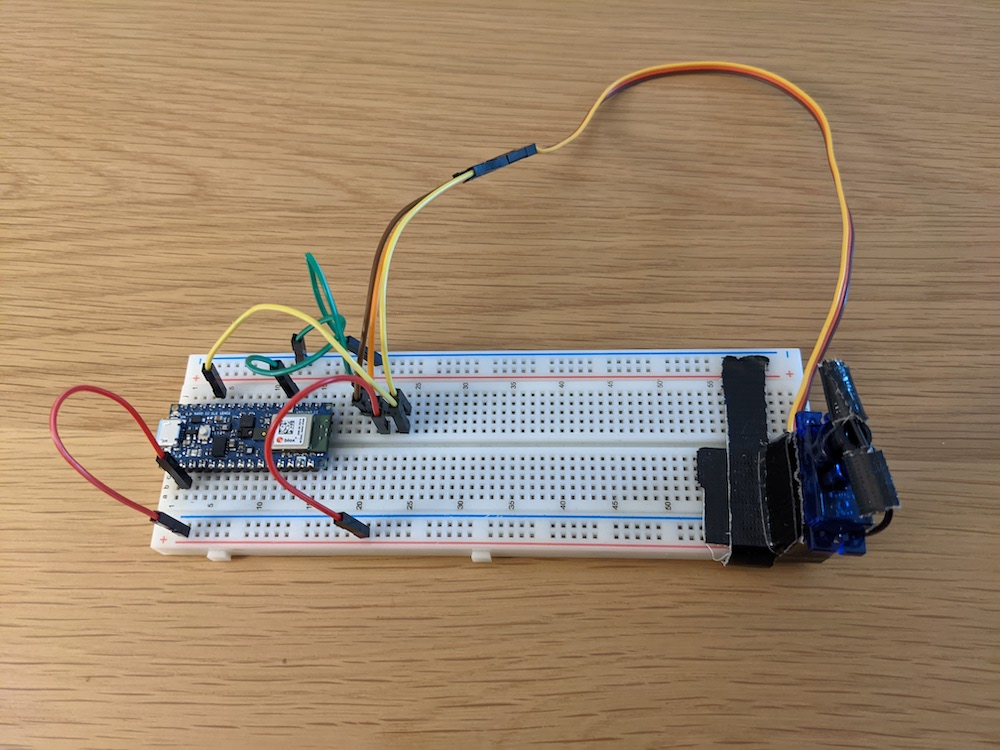
\includegraphics[width=0.75\textwidth]{images/desk.jpg}
	\caption{Desk at home}
	\label{fig:desk}
\end{figure}

This thesis is a collection of media arts instruments, using tiny machine learning, and with a strong emphasis on digital ethics and Do-It-Yourself (DIY). Its main audience is beginners and artists, and it is my hope that this work can inform the discourse and practice of a new generation of artists,  designers, educators, programmers, policy makers, activists, and enthusiasts.

Machine learning can be really difficult and often relies on proprietary software and hardware. They often need to be trained in borrowed and rented resources, such as the service Google Colab, which allows you to share and train ML models on the cloud. This thesis shows users how to build machine learning art systems that can circumvent this and allow for more control of their data.

Artists have an unprecedented access to new tools for making new tools and instruments, and this thesis intends to be a foundation for a new generation of instruments for manipulating audiovisual material, using machine learning. This approach is really exciting because it allows beginners and artists to train their instruments instead of programming them, by inputting data for tuning, instead of having to write lines of code and fixed thresholds for changing their behavior.

Machine learning algorithms are written by humans, and then trained on biased data, and they are deployed to the world, where they affect our lives. These imperfections are highlighted over the course of this thesis, by being explicit about the assumptions and quantizations performed when working with data.

TODO: Add example of biased dataset that is commonly used.

The proliferation of surveillance tools and now of microcontrollers allows for an even more pervasive surveillance and data leaks by governments and corporations. This thesis allows for beginners and artists to develop their own databases, by self sensing and surveillance. TODO: explain self-sensing and surveillance, and explain harms of surveillance, with an example.

Low power and repurposable
Tiny machine learning is defined as machine learning performed with low-power devices TODO: add citation or mention that it is my own definition. The proposal of media arts instruments that can run on little power, rechargeable batteries is a friendly use of resources for experimentation in arts. This is in contrast with the high power use and critique of other emerging fields such as Non Fungible Tokens (NFTs) and cryptoart. The proposal of these scriptable open source instruments allows for users to continuously tweak and modify their instruments, repurpose the hardware, and enable sharing.

TODO: Add a reference to an early tiny ML paper.

\section{Objectives}

With the release of TensorFlow Lite Micro, the TinyML Foundation, new avenues have been opened for creative expression using machine learning in microcontrollers.

TODO: Explain what is TensorfLow Lite Micro, what does it do, the same for TinyML Foundation

COMMENT: add in a paragraph here that combines the points you make in the first paragraphs -> the main contributions of YOUR thesis... which it seems is basically just addressing a bunch of the context section? Blakeley Payne's thesis does a good job of outlining contributions. It's also good to do here to understand where you are going

Homebrew examples, teach people how to build their own databases, and how to circumvent corporations view,

TODO: Terms and conditions comic book. If people were to read terms and conditions, it would take them X years

You can train an instrument to only detect your voice, your accent, your living conditions.

TODO: add blurb main inspiration about trail building and skatepark, and playpens, sandbox

TODO: add Marina Berry’s paper on playgrounds, child development

TODO: Technology and Public Art with Rafael Lozano-Hemmer | June 3, 2020
https://www.youtube.com/watch?v=QgVdEmqmuEE
36m28s
Rafael Lozano-Hemmer: “Face recognition needs to be banned in all applications except art.”

TODO: add Zoom example of garbage speech to text
TODO: Add in a glossary of terms to go over the basics of machine learning
TODO: Add contextual stories to frame each aspect
TODO: More pictures
TODO: Add how everything is public, even the errors
TODO: Raspberry Pi example, it’s cheap but it needs a lot of extra hardware to be used
TODO: Also add examples about April Fools Day and Terms and Conditions, about owning your soul
TODO: link https://www.youtube.com/watch?v=jOQ-9S3lOnM\&t=125s
TODO: Terms and conditions citation: (copied this in from my thesis, but check out McDonald and Cranor 2008) https://kb.osu.edu/handle/1811/72839 "Just considering privacy policies shown to people online in one year, it's been estimated that consumers would need approximately 244 hours to read, not skim, privacy policies shown to them in one calendar year."


\section{Outline}

This thesis will cover the following chapters:

\begin{enumerate}
        \item Chapter 2: Background: the inspiration and context of this thesis. TODO: add literature that informs my work.
    \item Chapter 3: Early experiments: my earlier work that led to this thesis, in the topics of media arts education, microcontrollers, and machine learning.
    \item Chapter 4: Tiny Trainable Instruments: description of design strategies for the software and hardware, description of the support team working on this thesis.
    \item Chapter 5: Project evaluation: user feedback, field notes.
    \item Chapter 6: Future work: next iterations of the instruments, and their proposed use for educators and artists.
  \end{enumerate}

\chapter{Tiny trainable instruments}

This chapter describes what this project is, its philosophy, design principles, and scope of this thesis project.

\section{Philosophy}


\section{Antidisciplinarity}

This project draws from different disciplines, all intertwined and in different capacities, including:

\begin{enumerate}
  \item Artificial intelligence
  \item Electrical engineering
  \item Computer science
  \item Media arts
  \item Music
\end{enumerate}

\section{Design principles}

\begin{enumerate}
  \item Cheap
  \item Private
  \item Open
  \item Hackable
\end{enumerate}

\subsection{Cheap}



\section{Technology}

This project is built with microcontrollers and 

This project is based on the Arduino Nano 33 BLE Sense microcontroller, and its software dependencies include the Arduino KNN library, the Arduino TensorFlow Lite Micro library, and Adafruit software libraries. 

\section{Open}

All examples included with this library were written with the aim of showing the fundamentals of how to build the instruments and different machine learning enabled manipulation of multimedia material, so that people could build on top of it and make it their own, by changing the values of variables and adding more functionalities.

\section{Philosophy and experience}

Throughout this project, the magic number was 3. The machine learning algorithms were hardcoded to be able to distinguish between 3 different categories: 3 colors, 3 physical gestures, 3 sound utterances.

\section{Inputs}

We are using the RGB color, proximity, gyroscope, accelerometer, and microphone sensors on the microcontroller, in order to capture the Inputs

\begin{enumerate}
  \item Color
  \item Gesture
  \item Speech
\end{enumerate}

\subsection{Color}

This approach uses the RGB color sensor from the microcontroller, with the auxiliary help from the proximity sensor, that is used to capture color information at a certain distance threshold.

The data is passed to a k-Nearest-Neighbor algorithm, programmed using the Arduino KNN library.

\subsection{Gesture}

This input uses the information from the Inertial Measurement Unit (IMU) of the microcontroller, including a gyroscope and accelerometer. It captures data after a certain threshold of movement is detected.

The data is passed to a TensorFlow neural network, programmed using the Arduino TensorFlow Lite library, and based on the included magic$\_$wand example.

\subsection{Speech}

This input uses the information from the microphone of the microcontroller.

The data is passed to a TensorFlow neural network, programmed using the Arduino TensorFlow Lite library, and based on the included micro$\_$speech example.

\section{Outputs}

The different outputs were picked, because of their low cost, ubiquity, and possibilities of expansion and combining them.

\subsection{Buzzer}

This output creates pitched sound, by using a PWM output.

\subsection{Servo motor}

This output creates movement and through that, rhythmic sounds.

The main inspiration for this output was the emerging use of motor-activated percussive instruments, such as the Polyend Perc.

\subsection{MIDI}

We wrote functionalities to manipulate MIDI instruments, and included examples to interface with some popular and cheap MIDI instruments, such as the Korg volca beats.

We included examples for rhythmic and melodic elements, using two very ubiquitous and inexpensive MIDI musical instruments, which are the Korg volca beats, and the Korg volca keys.

\subsection{Thermal printer}

A thermal printer is the basis for creating written and literary output, inspired by the field of computational poetry.

We used the popular Adafruit Thermal printer kit, which is documented on their website and includes a software library, distributed over GitHub and Arduino IDE, and also as a submodule on this project's TinyTrainable software library.

\section{Development}

This thesis has been developed with the invaluable help of undergrad researchers Peter Tone and Maxwell Wang.

They have cloned both repositories, the main one and the Arduino library one, and have continuously submitted pull requests with their contributions.

Peter Tone has helped with research in data structures, library writing, and we have shared back and forth code, going from experimental proofs of concepts, and has also helped with the design of the user-facing library.

Maxwell Wang has proofread the code, has ran the examples, and has helped with the writing of the documentation for self-learners and for the workshops.

We all share a Google Drive folder, where we all share notes about our research and development of the library and the educational material.

\section{Code}

This thesis is distributed as a repository, hosted on the GitHub platform, and available at https://github.com/montoyamoraga/tiny-trainable-instruments.

The auxiliary files, such as the LaTeX project for this document, and the auxiliary Jupyter notebooks, and documentation and tutorials are included on this repository.

The main software component of this project is the TinyTrainable library, available at https://github.com/montoyamoraga/TinyTrainable and also through the Arduino IDE.

The code included on this library is distributed on the folders:

\begin{enumerate}
  \item examples/
  \item src/
\end{enumerate}

\subsection{src/}

The source code for where there is a TinyTrainable.h and TinyTrainable.cpp file where we included all the basic functionality of the library. Additional subfolders include

\subsubsection{inputs/}

Base class Input and inherited classes for each one of the other inputs.

\subsubsection{outputs/}

Base class Output and inherited classes for each one of the other outputs.

\subsubsection{tensorflow/}

Auxiliary files, copied from the examples from the Arduino TensorFlow Lite that we are building on top of, and also from the newer TinyML library by the EdX team. These, unless otherwise noted, are included without modifications and distributed through the Apache License included on each file's headers.

\section{Opera of the Future projects}

During the development of this thesis, I have been fortunate to collaborate on different capacities with other thesis projects by classmates at Opera of the Future, which has directly inspired my work.

\subsection{Squishies, by Hannah Lienhard}

Squishies is Hannah Lienhard's master's thesis, and consists of a novel squishable interfaces for musical expression. We shared discussions about low-level sound design, code reusability, sound art education, digital instruments. We were part of a master's thesis working group, facilitated by Roya Moussapour with two other Media Lab classmates, where we workshopped drafts of our thesis. This practice and feedback has been critical in shaping the language and discourse of this thesis document.

\subsection{Fluid Music, by Charles Holbrow}

Fluid Music is Charles Holbrow's PhD thesis. It is a library for library design, documentation for contributors. The design of the interface, documentation, and scope of the thesis were a direct influence on the documentation and API coding style of this project.

Overall thoughts: I think it would be great if your Chapter 3 clearly led you to the design principles you lay out in Chapter 4. So, why is “open” important -> because of the collaborations or arduino libraries you used. Why is “cheap”/”privacy” -> coded bias and ability to tinker, etc.

\include{chap3}
\include{chap4}
\chapter{Project evaluation}

\section{Overview}

This thesis lives as a PDF document at the MIT library, as a software library with examples for Arduino, and as repositories on GitHub with all the source code and history of the project.

\section{Digital release}

The repositories are hosted on GitHub, to promote collaboration, and people can file issues and pull requests.

GitHub repository

Arduino library

PDF zine for explaining, reference as the PDF booklet for monome norns

\section{Audience engagement}


\section{Workshop}

For user testing and sharing this thesis, some workshops were conducted during TODO, with support from a grant at CAMIT for teaching the workshops in English in USA, and in Chile in Spanish, remotely over teleconferencing software and after being approved by the MIT COUHES TODO explain.

The workshop instructions are documented on the docs/ folder of the repository available at https://github.com/montoyamoraga/tiny-trainable-instruments

Each workshop consists of 2 sessions of 2 hours each, spread over a weekend.

On the first session we will first help people with installation of the software, and then move on to start wiring the materials on the electronic breadboard material. We will concentrate on the simpler examples with color input. We will also collect data of gesture and speech to create custom databases and use them to train other slow machine learning models, that will keep on running on the student's workshops after the workshop is over.

On the second session we will use the result of the trained models to create more advanced instruments that react to gesture and speech. We will also show the participants the other 
 
\section{Multimedia documentation}

TODO: upload a collection of examples made by people who came to the workshops, featuring the software library and what they learned.

\chapter{Conclusions}

In this thesis I have presented all the stages of the design and development of a software library for creating new standalone multimedia instruments using machine learning and microcontrollers, with a strong focus on AI ethics. The project includes software examples, hardware suggestions, educational material, and strategies for ethical off-cloud machine learning and creation of custom artisanal databases.

This thesis is also the basis for further research, including the creation of subsequent multimedia instruments and software, the writing of new courses and educational units at the intersection of arts, physical computing, interaction design, and computational ethics.

\section{Lessons learned}

so that future makers can learn from this process

Work with other people

Dont’ assume things

maybe appendix: 3 or 5 things i could do differenntly
maybe appendix: what could be different in a future without covid

\section{Contributions}

My contributions include 

\section{Future work}

\subsection{Hardware for new instruments}

TODO: right now this section is not a brief summary of what i’ve presented before, it is too detailed. Instead, quickly summarize what you've discussed in each chapter in no more than one paragraph per chapter and then switch to the impact of your work and future connections.

This project relies on a particular microcontroller, the Arduino Nano 33 BLE Sense. I used and Arduino board because of its popularity, availability, and software and community support.

The particular board's main draw for building multimedia instruments is its embedded sensors, including microphone, gyroscope, and camera. This embedding on the chip makes it more attractive than other boards, where users need to acquire, wire, and calibrate off-board sensors, making the process of capturing data more cumbersome and expensive in resources, adding additional barriers to instrument makers and prototypers. 

When this project started in 2020, and still today, this board was the only Arduino microcontroller supported by the Google TensorFlow Lite Micro library, for machine learning using microcontrollers, and it was heavily featured on the first promotional and educational material, which were the direct inspiration for this thesis, in terms of openness about the materials.

Microcontrollers come and go, most probably this board will be discontinued, and I hope this project can be adapted to other boards and architectures, particularly to other open source microcontrollers, including other Arduino boards, PJRC Teensy and Adafruit Circuit Playground, among others.

In terms of the outputs of the Tiny Trainable Instruments, I focused on creating many parallel multimedia approaches, including making sounds with piezo buzzers and MIDI, manipulating light with LEDs, creating movement and rhythm with servo motors, and printing text with thermal printers and screens. This is to appeal to a larger audience of artists and learners, interested in different mediums.

The Tiny Trainable Instruments are built with prototyping electronic breadboards, to make explicit their open-endedness, and to relate to a flux, instead of a fixed in state PCB, and a further state of this project would include the creation of custom boards with fixed wiring, and of enclosures and packaging.


\subsection{Software for new instruments}

This thesis has been published as an open source software library for Arduino. It promotes modularity and adaptability, where a Tiny Trainable Instrument can be any combination of the multiple inputs and outputs.

The file structure of the source code and the software dependencies of this library was also built with flexibility in mind, to encourage the remix and adaptation of this library to further projects.

A particular challenging aspect of this project, is the breadth of the disciplines combined, and its novel application of machine learning in microcontrollers. As discussed in previous chapters, there is a trend and new wave of builders and makers creating standalone multimedia instruments, based on open operating systems like Linux, and/or different microcontrollers. 

Despite the existence of artists and makers building standalone computational instruments, these skills are still hard to acquire. Additionally, the principles of this project, including being as cheap as possible, and as open as possible, are designed to encourage experimentation and hacking, but also can pose additional challenges. I hope this project encourages people to learn how to make instruments, and also engages in discourse about the creation of new curricula for the next generation of instrument makers and artists.

Another particular challenging aspect of writing software for multimedia instruments includes the licensing. The dependencies of this software are mostly other libraries by Arduino, Google, Adafruit, and with different licenses including public domain, MIT, and Apache. I hope this document helps to navigate these legal complexities and that this project helps artists and enthusiasts to navigate this landscape and overcome these barriers.

\subsection{Educational impact}

This project was built to inspire and celebrate a new generation of coursework, workshops, books, and 

I hope that this thesis project is ad

I hope that this thesis project is adopted by educators, to introduce students to machine learning, physical computing, media arts, and ethics.

Many sections of this project could be adapted to further existing curricula for music, rhythm, ethics, computer science, and to create a new wave of instrument makers and media artists.

TODO: maybe add potential future users. Talk about how I envision this project being used in these contexts.

\appendix
\chapter{Context}

During this thesis I had this particular context:

\section{Language}

My native language is Spanish, and this thesis was written in English.

\section{Social}

This thesis was written during the COVID19 pandemic, during the longest stretch I have had of not visiting my home country Chile, or leaving USA and its east coast, and not working on a shared office, or living with roommates, or seeing family, limiting my physical interactions to mostly a handful of friends and toi the internet.

\section{Location}

Written in Boston MA, New York City NY, Mt Airy MD, between November 2020 and July 2021.

\section{Software}

This thesis document was written using LaTeX and the Microsoft Visual Studio Code editor.

The TinyTrainable library was written in C++, and packaged as an Arduino library, relying on open source library dependencies by Arduino, Adafruit, and Google.

The auxiliary code is a mix of Python scripts, Jupyter notebooks, and shell scripts.

The documentation was written using Markdown.

The workshops were taught using the videoconferencing software Zoom, and organized via Google Forms.

\section{Hardware}

This project was written on a 2017 Macbook Air 13-inch, running macOS Catalina.

The software library and the software examples were written to be deployed on the Arduino Nano 33 BLE Sense microcontroller.

\newpage

\chapter{Alternate worlds}

These are some aspects I would do differently I could start again:

These are some aspects I would do differently if COVID19 hadn't happened:

\include{biblio}
\end{document}
